\chapter{Beispiele}

%% ---------------------------------------------
%% Abbildung
%% ---------------------------------------------
\section{Abbildung}
In der Abbildung \ref{fig_example} ...

\begin{figure}[!h]
    \centering
    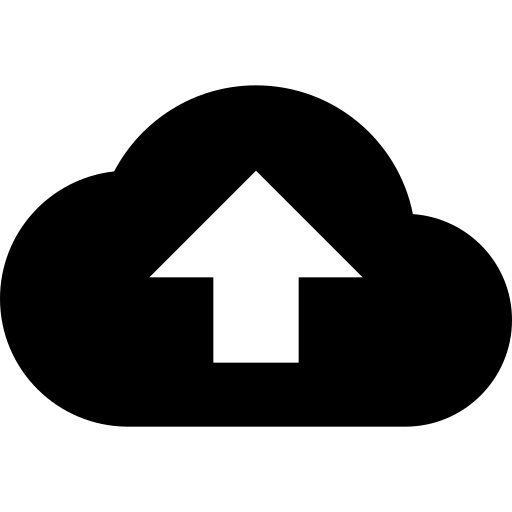
\includegraphics[width=\textwidth]{img/example_image.png}
    \caption{Ein wundervolles Bild in ganzer Breite}
    \label{fig_example}
\end{figure}

Die Abbildung \ref{fig_example_halfsize} hat die 50 Prozent Breite ...

\begin{figure}[h!]
    \centering
    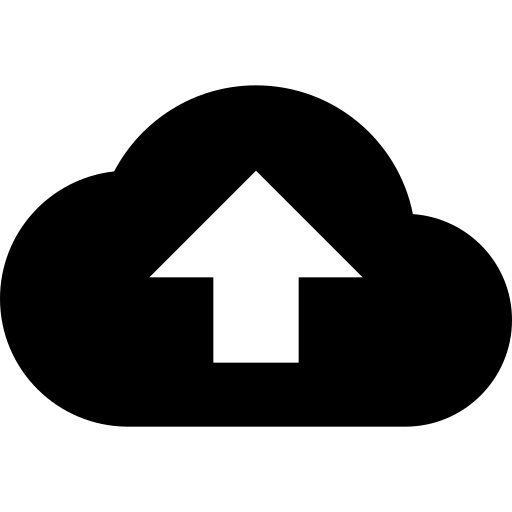
\includegraphics[width=0.5\textwidth]{img/example_image.png}
    \caption[Kurzbeschreibung für Abbildungsverzeichnis]{Ein wundervolles Bild in 50\% Breite}
    \label{fig_example_halfsize}
\end{figure}

%% ---------------------------------------------
%% Abkürzung
%% ---------------------------------------------
\section{Abkürzung}
Eine Verlinkung zur \acs{Abkürzung} ist auch möglich. Jedoch gibt es bei Umlauten Probleme...

%% ---------------------------------------------
%% Anführungszeichen
%% ---------------------------------------------
\section{Anführungszeichen}
\glqq Anführungszeichen\grqq{} können mit \mintinline{latex}{\glqq} für das linke und \mintinline{latex}{\grqq{}} für das rechte Anführungszeichen ergänzt werden.

%% ---------------------------------------------
%% Auflistung
%% ---------------------------------------------
\section{Auflistung}
In der folgenden Auflistung...
\begin{itemize}
    \setlength\itemsep{-1em}
    \item erstes Stichwort
    \item zweites Stichwort
    \item dritte Stichwort
\end{itemize}

Eine Auflistung mit einem anderen Abstand zwischen den Punkten...
\begin{itemize}
    \setlength\itemsep{-0.5em}
    \item erstes Stichwort
    \item zweites Stichwort
    \item dritte Stichwort
\end{itemize}

%% ---------------------------------------------
%% Kurze Tabelle
%% ---------------------------------------------
\section{Kurze Tabelle}
In der Tabelle \ref{tbl_example_table} ...

\begin{table}[!h]
    \centering
    \begin{tabular}{l|ll}
        Datensatz 1     & Wert 1    & Einheit \\
        Datensatz 2     & Wert 2    & Einheit \\ \hline
        $\sum$          & Summe     & Einheit \\
    \end{tabular}
    \caption{Beispiel für eine Tabelle}
    \label{tbl_example_table}
\end{table}

%% ---------------------------------------------
%% Lange Tabelle
%% ---------------------------------------------
\section{Lange Tabelle}
Eine lange Tabelle mit einem alternativen Text für das Tabellenverzeichnis...
\begin{longtable}{p{0.5\linewidth} p{0.5\linewidth}}
    \hline
    Lorem ipsum dolor sit amet, consetetur sadipscing elitr, sed diam nonumy eirmod tempor invidunt ut labore et dolore magna aliquyam erat, sed diam voluptua. &
    Lorem ipsum dolor sit amet, consetetur sadipscing elitr, sed diam nonumy eirmod tempor invidunt ut labore et dolore magna aliquyam erat, sed diam voluptua. \\
    \hline
    Lorem ipsum dolor sit amet, consetetur sadipscing elitr, sed diam nonumy eirmod tempor invidunt ut labore et dolore magna aliquyam erat, sed diam voluptua. &
    Lorem ipsum dolor sit amet, consetetur sadipscing elitr, sed diam nonumy eirmod tempor invidunt ut labore et dolore magna aliquyam erat, sed diam voluptua. \\
    \hline
    Lorem ipsum dolor sit amet, consetetur sadipscing elitr, sed diam nonumy eirmod tempor invidunt ut labore et dolore magna aliquyam erat, sed diam voluptua. &
    Lorem ipsum dolor sit amet, consetetur sadipscing elitr, sed diam nonumy eirmod tempor invidunt ut labore et dolore magna aliquyam erat, sed diam voluptua. \\
    \hline
\caption[Alternativer kürzerer Text für eine Caption]{Hier eine lange Tabelle mit zwei Spalten (je 50\% Breite). Diese könnte auch über mehrere Seiten gehen}
\label{tbl_longtable}
\end{longtable}

%% ---------------------------------------------
%% PDF
%% ---------------------------------------------
\section{PDF}
Mit dem Compiler \textit{pdfLaTeX} ist es möglich andere PDF-Dokumente wie ein Bild einzubinden (siehe \ref{fig_example_pdf}).

\begin{figure}[h!]
    \centering
    
\includegraphics[width=0.5\textwidth]{img/Example.pdf}
    \caption[Beispiel für PDF-Einbindung]{Einbinden eines PDFs in LaTeX}
    \label{fig_example_pdf}
\end{figure}

%% ---------------------------------------------
%% Quellcode
%% ---------------------------------------------
\section{Quellcode}
Quellcode kann als Block oder im Fließtext stehen. Der Ausdruck \mintinline{python}{print(x**2)} ist ein Beispiel für Inline-Quelltext.

Für langen Inline-Quellcode wird kein automatischer Zeilenumbruch eingefügt: \mintinline{python}{[ x if x mod 2 else x*100 for x in range(1, 10) ]}.
Es handelt sich dabei um ein bekanntes Problem (\url{https://tex.stackexchange.com/questions/419934/breaklines-doesnt-work-with-mintinline} ). Beim Einfügen von Inline-Quellcode muss ggf. manuell ein Zeilenumbruch eingefügt werden (\mintinline{latex}{\\}).

Folgender Code-Block taucht nicht im Code-Verzeichnis auf:
\begin{minted}{json}
{   
    "id" : 1234,  
    "field1": "hallo",  
    "field2" : "welt"
}
\end{minted}

Folgender Code-Block taucht im Code-Verzeichnis auf: \\
\begin{code}{json}{Eine tolle Unterschrift von einem JSON-Codeblock}{code:json-label}
{   
    "id" : 1234,
    "field1": "hallo",
    "field2" : "welt"
}
\end{code}

Codeblöcke können mit \mintinline{latex}{\ref{<labelname>}} referenziert werden, ungefähr so: \ref{code:json-label}.

%% ---------------------------------------------
%% Referenzen
%% ---------------------------------------------
\section{Referenzen}\label{sec_referenzen}
Der Name einer Referenz wird mit \mintinline{LaTeX}{\label{name_der_referenz}} festgelegt. Für einen Abschnitt zum Beispiel: \mintinline{LaTeX}{\section{Referenzen}\label{sec_referenzen}}.

Referenzen auf Bilder, Gleichungen, Kapitel oder andere Elemente können mit \mintinline{LaTeX}{\ref{name_der_referenz}} eingefügt werden. \\
\textbf{Zum Beispiel:} Abbildung \ref{fig_example_pdf}, Abschnitt \ref{sec_referenzen} \\
\textbf{Quellcode für Beispiel:} \mintinline{LaTeX}{Abbildung \ref{fig_example_pdf}, Abschnitt \ref{sec_referenzen}}

Um automatisch das Präfix \glqq Abbildung\grqq{}, \glqq Gleichung\grqq{} oder \glqq  Abschnitt\grqq{} zu erhalten, kann der Befehl \mintinline{LaTeX}{\autoref{name_der_referenz}} genutzt werden. \\
\textbf{Zum Beispiel:} \autoref{fig_example_pdf}, \autoref{sec_referenzen} \\
\textbf{Quellcode für Beispiel:} \mintinline{LaTeX}{\autoref{fig_example_pdf}, \autoref{sec_referenzen}}

%% ---------------------------------------------
%% Zitieren
%% ---------------------------------------------
\section{Zitieren}
Wie durch Quelle \cite{Nobody05} oder \cite{Nobody06} belegt ist...

Angabe von Seitenzahl für die Quelle \cite[S. 5ff]{Nobody07}
